\documentclass[]{report}
\usepackage{lmodern}
\usepackage{amssymb,amsmath}
\usepackage{ifxetex,ifluatex}
\usepackage{fixltx2e} % provides \textsubscript
\ifnum 0\ifxetex 1\fi\ifluatex 1\fi=0 % if pdftex
  \usepackage[T1]{fontenc}
  \usepackage[utf8]{inputenc}
\else % if luatex or xelatex
  \ifxetex
    \usepackage{mathspec}
  \else
    \usepackage{fontspec}
  \fi
  \defaultfontfeatures{Ligatures=TeX,Scale=MatchLowercase}
\fi
% use upquote if available, for straight quotes in verbatim environments
\IfFileExists{upquote.sty}{\usepackage{upquote}}{}
% use microtype if available
\IfFileExists{microtype.sty}{%
\usepackage{microtype}
\UseMicrotypeSet[protrusion]{basicmath} % disable protrusion for tt fonts
}{}
\usepackage{hyperref}
\hypersetup{unicode=true,
            pdftitle={Homework Part 2},
            pdfauthor={Vinicio Haro; Sang Yoon (Andy) Hwang; Julian McEachern; Jeremy O'Brien; Bethany Poulin},
            pdfborder={0 0 0},
            breaklinks=true}
\urlstyle{same}  % don't use monospace font for urls
\usepackage{color}
\usepackage{fancyvrb}
\newcommand{\VerbBar}{|}
\newcommand{\VERB}{\Verb[commandchars=\\\{\}]}
\DefineVerbatimEnvironment{Highlighting}{Verbatim}{commandchars=\\\{\}}
% Add ',fontsize=\small' for more characters per line
\usepackage{framed}
\definecolor{shadecolor}{RGB}{248,248,248}
\newenvironment{Shaded}{\begin{snugshade}}{\end{snugshade}}
\newcommand{\AlertTok}[1]{\textcolor[rgb]{0.94,0.16,0.16}{#1}}
\newcommand{\AnnotationTok}[1]{\textcolor[rgb]{0.56,0.35,0.01}{\textbf{\textit{#1}}}}
\newcommand{\AttributeTok}[1]{\textcolor[rgb]{0.77,0.63,0.00}{#1}}
\newcommand{\BaseNTok}[1]{\textcolor[rgb]{0.00,0.00,0.81}{#1}}
\newcommand{\BuiltInTok}[1]{#1}
\newcommand{\CharTok}[1]{\textcolor[rgb]{0.31,0.60,0.02}{#1}}
\newcommand{\CommentTok}[1]{\textcolor[rgb]{0.56,0.35,0.01}{\textit{#1}}}
\newcommand{\CommentVarTok}[1]{\textcolor[rgb]{0.56,0.35,0.01}{\textbf{\textit{#1}}}}
\newcommand{\ConstantTok}[1]{\textcolor[rgb]{0.00,0.00,0.00}{#1}}
\newcommand{\ControlFlowTok}[1]{\textcolor[rgb]{0.13,0.29,0.53}{\textbf{#1}}}
\newcommand{\DataTypeTok}[1]{\textcolor[rgb]{0.13,0.29,0.53}{#1}}
\newcommand{\DecValTok}[1]{\textcolor[rgb]{0.00,0.00,0.81}{#1}}
\newcommand{\DocumentationTok}[1]{\textcolor[rgb]{0.56,0.35,0.01}{\textbf{\textit{#1}}}}
\newcommand{\ErrorTok}[1]{\textcolor[rgb]{0.64,0.00,0.00}{\textbf{#1}}}
\newcommand{\ExtensionTok}[1]{#1}
\newcommand{\FloatTok}[1]{\textcolor[rgb]{0.00,0.00,0.81}{#1}}
\newcommand{\FunctionTok}[1]{\textcolor[rgb]{0.00,0.00,0.00}{#1}}
\newcommand{\ImportTok}[1]{#1}
\newcommand{\InformationTok}[1]{\textcolor[rgb]{0.56,0.35,0.01}{\textbf{\textit{#1}}}}
\newcommand{\KeywordTok}[1]{\textcolor[rgb]{0.13,0.29,0.53}{\textbf{#1}}}
\newcommand{\NormalTok}[1]{#1}
\newcommand{\OperatorTok}[1]{\textcolor[rgb]{0.81,0.36,0.00}{\textbf{#1}}}
\newcommand{\OtherTok}[1]{\textcolor[rgb]{0.56,0.35,0.01}{#1}}
\newcommand{\PreprocessorTok}[1]{\textcolor[rgb]{0.56,0.35,0.01}{\textit{#1}}}
\newcommand{\RegionMarkerTok}[1]{#1}
\newcommand{\SpecialCharTok}[1]{\textcolor[rgb]{0.00,0.00,0.00}{#1}}
\newcommand{\SpecialStringTok}[1]{\textcolor[rgb]{0.31,0.60,0.02}{#1}}
\newcommand{\StringTok}[1]{\textcolor[rgb]{0.31,0.60,0.02}{#1}}
\newcommand{\VariableTok}[1]{\textcolor[rgb]{0.00,0.00,0.00}{#1}}
\newcommand{\VerbatimStringTok}[1]{\textcolor[rgb]{0.31,0.60,0.02}{#1}}
\newcommand{\WarningTok}[1]{\textcolor[rgb]{0.56,0.35,0.01}{\textbf{\textit{#1}}}}
\usepackage{graphicx,grffile}
\makeatletter
\def\maxwidth{\ifdim\Gin@nat@width>\linewidth\linewidth\else\Gin@nat@width\fi}
\def\maxheight{\ifdim\Gin@nat@height>\textheight\textheight\else\Gin@nat@height\fi}
\makeatother
% Scale images if necessary, so that they will not overflow the page
% margins by default, and it is still possible to overwrite the defaults
% using explicit options in \includegraphics[width, height, ...]{}
\setkeys{Gin}{width=\maxwidth,height=\maxheight,keepaspectratio}
\IfFileExists{parskip.sty}{%
\usepackage{parskip}
}{% else
\setlength{\parindent}{0pt}
\setlength{\parskip}{6pt plus 2pt minus 1pt}
}
\setlength{\emergencystretch}{3em}  % prevent overfull lines
\providecommand{\tightlist}{%
  \setlength{\itemsep}{0pt}\setlength{\parskip}{0pt}}
\setcounter{secnumdepth}{0}

%%% Use protect on footnotes to avoid problems with footnotes in titles
\let\rmarkdownfootnote\footnote%
\def\footnote{\protect\rmarkdownfootnote}

%%% Change title format to be more compact
\usepackage{titling}

% Create subtitle command for use in maketitle
\providecommand{\subtitle}[1]{
  \posttitle{
    \begin{center}\large#1\end{center}
    }
}

\setlength{\droptitle}{-2em}

  \title{Homework Part 2}
    \pretitle{\vspace{\droptitle}\centering\huge}
  \posttitle{\par}
    \author{Vinicio Haro \\ Sang Yoon (Andy) Hwang \\ Julian McEachern \\ Jeremy O'Brien \\ Bethany Poulin}
    \preauthor{\centering\large\emph}
  \postauthor{\par}
    \date{}
    \predate{}\postdate{}
  
% set plain style for page numbers
\pagestyle{plain}
\raggedbottom

% change font
\usepackage{fontspec}
\setmainfont{Arial}

% create color block quotes
\usepackage[dvipsnames]{xcolor}
\definecolor{navyblue}{RGB}{16, 52, 166}
\definecolor{stealblue}{RGB}{72, 90, 122}
\usepackage{tcolorbox}     
\newtcolorbox{question}[1]{colback=white, colframe=navyblue ,fonttitle=\bfseries, title=#1}

\newtcolorbox{subquestion}[1]{colback=white,colframe=white, coltitle=navyblue!75!black, detach title, before upper={\tcbtitle\quad\hangindent7mm}, title={#1},fonttitle=\bfseries, fontupper=\bfseries}


\usepackage{xcolor}
\usepackage{sectsty}
\usepackage{etoolbox}
\usepackage{titling}

\usepackage{titling}
\pretitle{\begin{flushright}\Huge\color{navyblue}\textbf}
\posttitle{\par\Large\color{gray}Data 624 - Predictive Analytics\linebreak 16 December 2019\end{flushright}}
\preauthor{\begin{flushright}\large \lineskip 0.5em\textbf{Group Members:}\linebreak\textit}
\postauthor{\par\end{flushright}}
\predate{\begin{flushright}\large}
\postdate{\par\end{flushright}}




% remove "chapter" from chapter title
\usepackage{titlesec}
\titleformat{\chapter}
  {\normalfont\color{navyblue}\LARGE\bfseries}{\thechapter}{1em}{}
\titlespacing*{\chapter}{0pt}{3.5ex plus 1ex minus .2ex}{2.3ex plus .2ex}


% margins
\usepackage[margin=1in]{geometry}

% kable 
\usepackage{tabu}
\usepackage{float} 
\usepackage{booktabs}
\usepackage[font={color=navyblue,bf}]{caption}

% multicolumn
\usepackage{multicol}
\usepackage{booktabs}
\usepackage{longtable}
\usepackage{array}
\usepackage{multirow}
\usepackage{wrapfig}
\usepackage{float}
\usepackage{colortbl}
\usepackage{pdflscape}
\usepackage{tabu}
\usepackage{threeparttable}
\usepackage{threeparttablex}
\usepackage[normalem]{ulem}
\usepackage{makecell}
\usepackage{xcolor}

\begin{document}
\maketitle

{
\setcounter{tocdepth}{2}
\tableofcontents
}
\hypertarget{Overview}{%
\chapter*{Getting Started}\label{Overview}}
\addcontentsline{toc}{chapter}{Getting Started}

\hypertarget{overview}{%
\section{Overview}\label{overview}}

Include details on our process in creating this document.

\hypertarget{dependencies}{%
\section{Dependencies}\label{dependencies}}

\begin{Shaded}
\begin{Highlighting}[]
\CommentTok{# Data Wrangling}
\KeywordTok{library}\NormalTok{(AppliedPredictiveModeling)}
\KeywordTok{library}\NormalTok{(mice)}
\KeywordTok{library}\NormalTok{(caret)}
\KeywordTok{library}\NormalTok{(tidyverse)}
\KeywordTok{library}\NormalTok{(pls)}
\KeywordTok{library}\NormalTok{(caTools)}
\KeywordTok{library}\NormalTok{(mlbench)}
\KeywordTok{library}\NormalTok{(stringr)}

\CommentTok{# Formatting}
\KeywordTok{library}\NormalTok{(default)}
\KeywordTok{library}\NormalTok{(knitr)}
\KeywordTok{library}\NormalTok{(kableExtra)}

\CommentTok{# Plotting}
\KeywordTok{library}\NormalTok{(ggplot2)}
\KeywordTok{library}\NormalTok{(grid)}
\KeywordTok{library}\NormalTok{(ggfortify)}
\KeywordTok{library}\NormalTok{(gridExtra)}
\end{Highlighting}
\end{Shaded}

\newpage

\hypertarget{AS-1}{%
\chapter*{Assignment 1}\label{AS-1}}
\addcontentsline{toc}{chapter}{Assignment 1}

\addcontentsline{toc}{subsection}{Kuhn and Johnson 6.3}

\begin{question}{Kuhn and Johnson 6.3}A chemical manufacturing process for a pharmaceutical product was discussed in Sect.1.4. In this problem, the objective is to understand the relationship between biological measurements of the raw materials (predictors), measurements of the manufacturing process (predictors), and the response of product yield. Biological predictors cannot be changed but can be used to assess the quality of the raw material before processing. On the other hand, manufacturing process predictors can be changed in the manufacturing process. Improving product yield by 1\% will boost revenue by approximately one hundred thousand dollars per batch:\end{question}

\begin{subquestion}{(a).}Start R and use these commands to load the data:
\end{subquestion}

\begin{Shaded}
\begin{Highlighting}[]
\KeywordTok{data}\NormalTok{(}\StringTok{"ChemicalManufacturingProcess"}\NormalTok{)}
\end{Highlighting}
\end{Shaded}

The matrix processPredictors contains the 57 predictors (12 describing
the input biological material and 45 describing the process predictors)
for the 176 manufacturing runs. yield contains the percent yield for
each run.

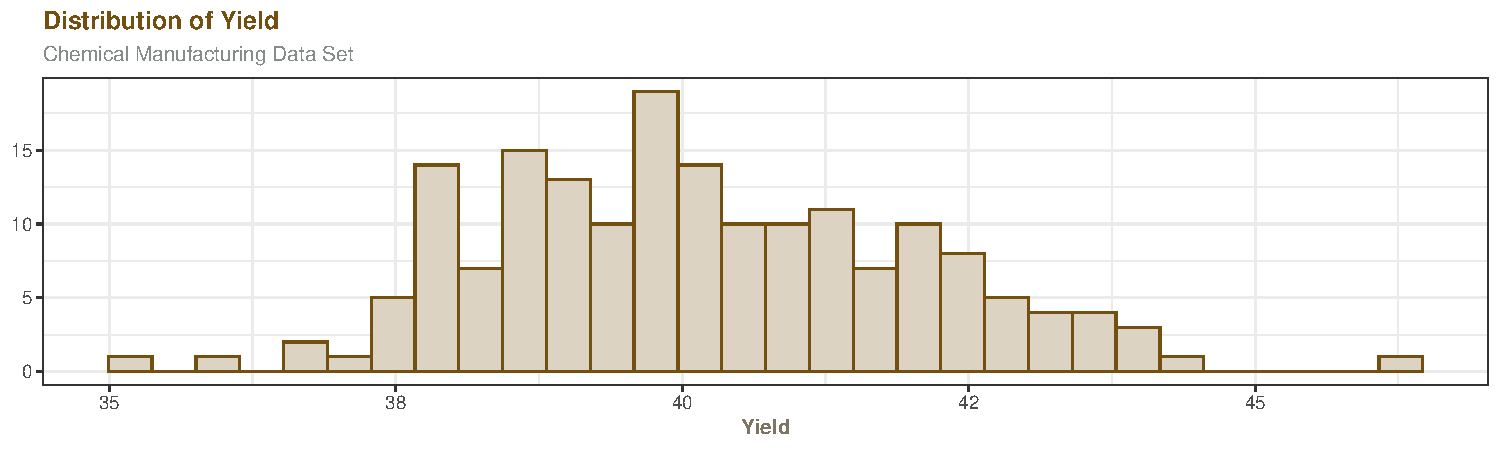
\includegraphics{Homework-Two_files/figure-latex/kj-6.3a-plot-1.pdf}

\begin{subquestion}{(b).} A small percentage of cells in the predictor set contain missing values. Use an imputation function to fill in these missing values (e.g., see Sect. 3.8). 
\end{subquestion}

\texttt{ManufacturingProcess03} has the largest volume of missing data
followed by \texttt{ManufacturingProcess11}. Given that each variable
has less than 25\% of data missing, we should introduce methods of
imputation. For our purposes, we will use the MICE method. MICE is
formally known as Multiple Imputation with Chained Equations. On a high
level, MICE is built off a tehcnique known as the Gibbs sampler.

The Gibbs sampler is a Markov chain based on Monte Carlo. MICE iterates
drawing estimates of missing values and parameters related to the
distribution of said variables. Chained equations are generally faster
than the monte carlo based Gibbs sampler. MICE has 5 imputations listed
as its default. predictive mean matching is also a default method for
MICE. PMM does a better job at keeping non-linear relationships within
individual variables.

In addition to MICE, we drop variables that have near zero variance,
however we point out that only one variable was dropped. We still
include it as a process step to follow the literature's specifications.
After completing MICE, we no longer had missing data in our set. We
examined other imputation methods such as KNN but determined that there
was no significant change in the summary statistics across different
imputation methods.

\begin{table}[H]

\caption{\label{tab:kj-6.3b}Variables with Missing Values}
\centering
\fontsize{8}{10}\selectfont
\begin{tabular}{lr>{\bfseries\raggedright\arraybackslash}p{0.1cm}lr}
\toprule
\textbf{Predictor} & \textbf{n} & \textbf{ } & \textbf{Predictor} & \textbf{n}\\
\midrule
\rowcolor{gray!6}  ManufacturingProcess03 & 15 &  & ManufacturingProcess02 & 3\\
ManufacturingProcess11 & 10 &  & ManufacturingProcess06 & 2\\
\rowcolor{gray!6}  ManufacturingProcess10 & 9 &  & ManufacturingProcess01 & 1\\
ManufacturingProcess25 & 5 &  & ManufacturingProcess04 & 1\\
\rowcolor{gray!6}  ManufacturingProcess26 & 5 &  & ManufacturingProcess05 & 1\\
\addlinespace
ManufacturingProcess27 & 5 &  & ManufacturingProcess07 & 1\\
\rowcolor{gray!6}  ManufacturingProcess28 & 5 &  & ManufacturingProcess08 & 1\\
ManufacturingProcess29 & 5 &  & ManufacturingProcess12 & 1\\
\rowcolor{gray!6}  ManufacturingProcess30 & 5 &  & ManufacturingProcess14 & 1\\
ManufacturingProcess31 & 5 &  & ManufacturingProcess22 & 1\\
\addlinespace
\rowcolor{gray!6}  ManufacturingProcess33 & 5 &  & ManufacturingProcess23 & 1\\
ManufacturingProcess34 & 5 &  & ManufacturingProcess24 & 1\\
\rowcolor{gray!6}  ManufacturingProcess35 & 5 &  & ManufacturingProcess40 & 1\\
ManufacturingProcess36 & 5 &  & ManufacturingProcess41 & 1\\
\bottomrule
\end{tabular}
\end{table}

\begin{subquestion}{(c).} Split the data into a training and a test set, pre-process the data, and tune a model of your choice from this chapter. What is the optimal value of the performance metric? 
\end{subquestion}

We will build a PLS model also known as partial least squares. PLS is a
statistical method that fits a linear regression model by projecting the
feature variables and response variable to some new space via a mapping
function. Because of this projection mechanisim, for both predictors and
the response, the method becomes bilinear or simply known as linear with
respect to to each of the variable types. PLS also has certain
advantages over other methods such as being more robust to dealing with
issues arising from multicolinearity.

For our PLS model, we partitioned the data by taking 80\% of the data as
training and the remaining 20\% as testing subsets. We also apply center
and scaling arguments set to true. We built a standard PLS model and
evaluated the root mean summary areas to determine the optimal number of
components to select. We generate performance metrics for our best tune
below:

\begin{table}[H]

\caption{\label{tab:kj-6.3c}PLS Performance Metrics on Training Subset}
\centering
\fontsize{8}{10}\selectfont
\begin{tabular}{rrr}
\toprule
\textbf{RMSE} & \textbf{Rsquared} & \textbf{MAE}\\
\midrule
\rowcolor{gray!6}  1.5626 & 0.3953 & 1.1845\\
\bottomrule
\end{tabular}
\end{table}

Our Baseline PLS model generates a RMSE of 1.56. In addition, the model
captures 39.53 \% of data variability. We include the visualizations
pertaining to the train set cross-validation RMSE tunes and a plot
comparing the observed and predicted outcome from our model.

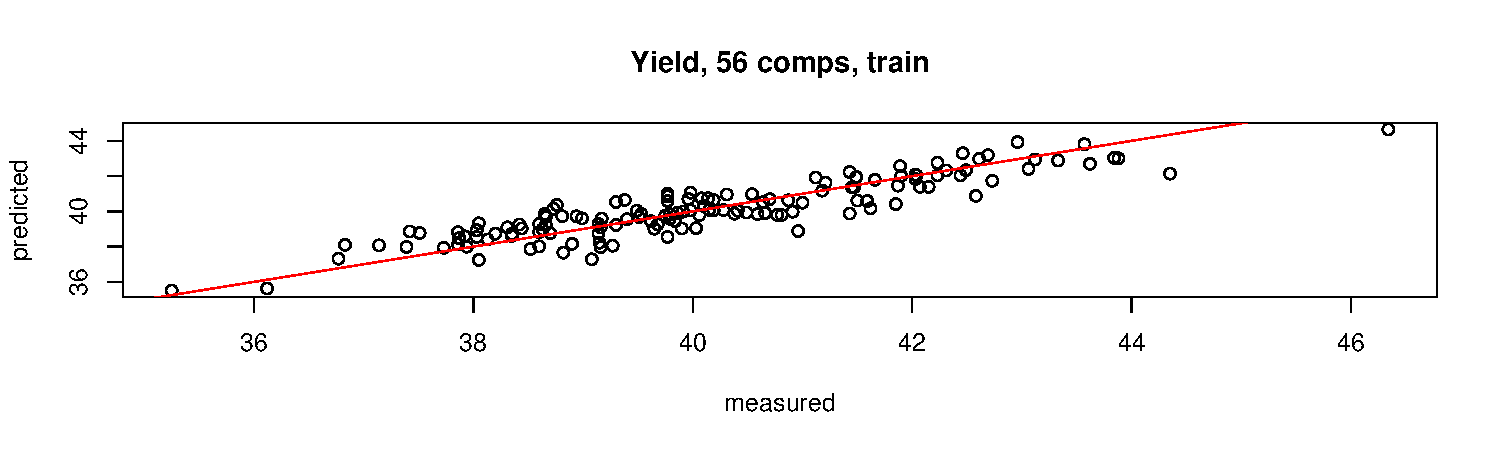
\includegraphics{Homework-Two_files/figure-latex/kj-6.3c2-1.pdf}

\begin{subquestion}{(d).} Predict the response for the test set. What is the value of the performance metric and how does this compare with the resampled performance metric on the training set? 
\end{subquestion}

We see a decreased R squared against the test data with 22\% of the data
variability accounted for. We also see the RMSE decrease to 1.52 from
our training results of 1.56. There is also a slight increase in the
MAE.

\begin{table}[H]

\caption{\label{tab:kj-6.3d-1}PLS Performance Metrics on Test Subset}
\centering
\fontsize{8}{10}\selectfont
\begin{tabular}{rrr}
\toprule
\textbf{RMSE} & \textbf{Rsquared} & \textbf{MAE}\\
\midrule
\rowcolor{gray!6}  1.5222 & 0.2212 & 1.2885\\
\bottomrule
\end{tabular}
\end{table}

We also plotted the observed and predicted values from our test set
against each other below. The deviation from the fitted line tells us
that our selected linear model may not provide the best predictions for
\texttt{Yield}.

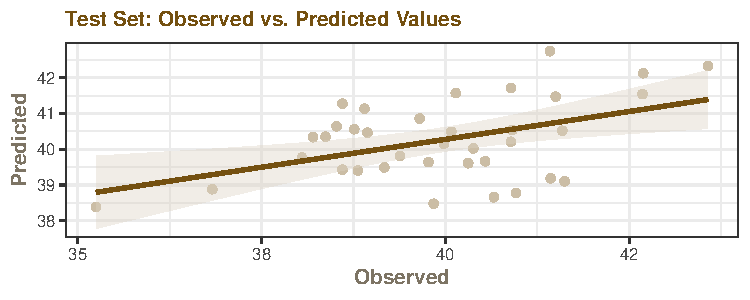
\includegraphics{Homework-Two_files/figure-latex/kj-6.3d-2-1.pdf}

\begin{subquestion}{(e).} Which predictors are most important in the model you have trained? Do either the biological or process predictors dominate the list? 
\end{subquestion}

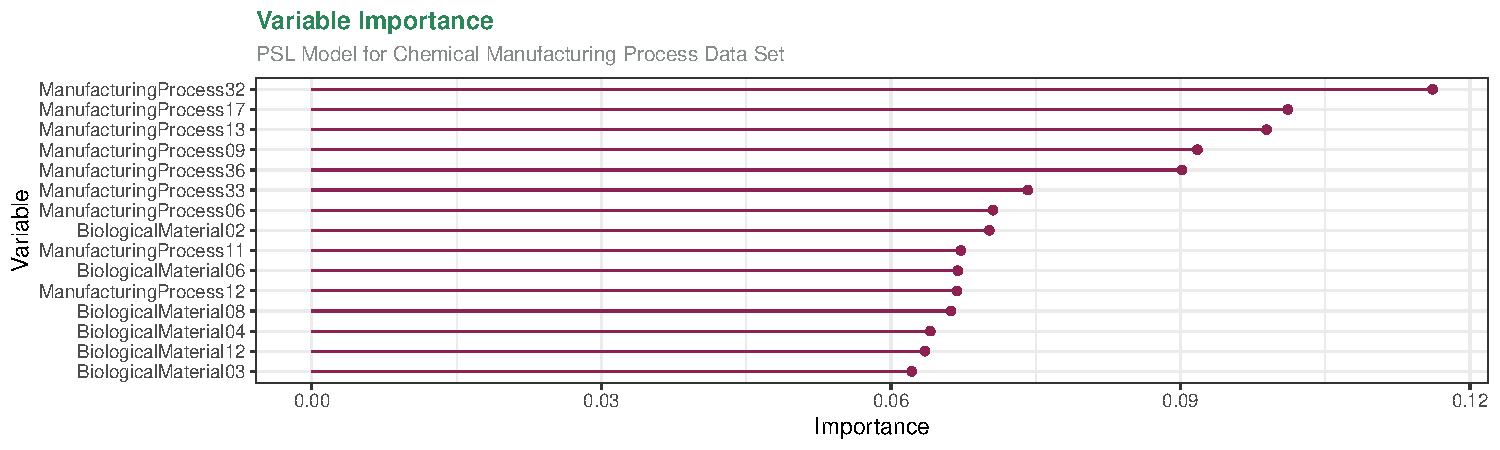
\includegraphics{Homework-Two_files/figure-latex/kj-6.3e-1.pdf}

VarImp allows us to identify the variables by name and compute their
importance. \texttt{ManufacturingProcess32} was flagged as the most
important predictor overall and within the group of other Manufacturing
Process variables. \texttt{BiologicalMaterial06} ranked second and was
the most important variable within the BiologicalMaterial group. The
variable importance rankings are mixed with 8 variables belonging to
Biology and 7 by Manufacturing Process within the top \(15\) predictors.

\begin{subquestion}{(f).} Explore the relationships between each of the top predictors and the response. How could this information be helpful in improving yield in future runs of the manufacturing process?
\end{subquestion}

We used a scatter plot to visualize the relationship between our top
five important predictors against our response variable, \texttt{Yield}.
All but \texttt{ManufacturingProcess32} show a moderate positive, linear
relationship with yield.

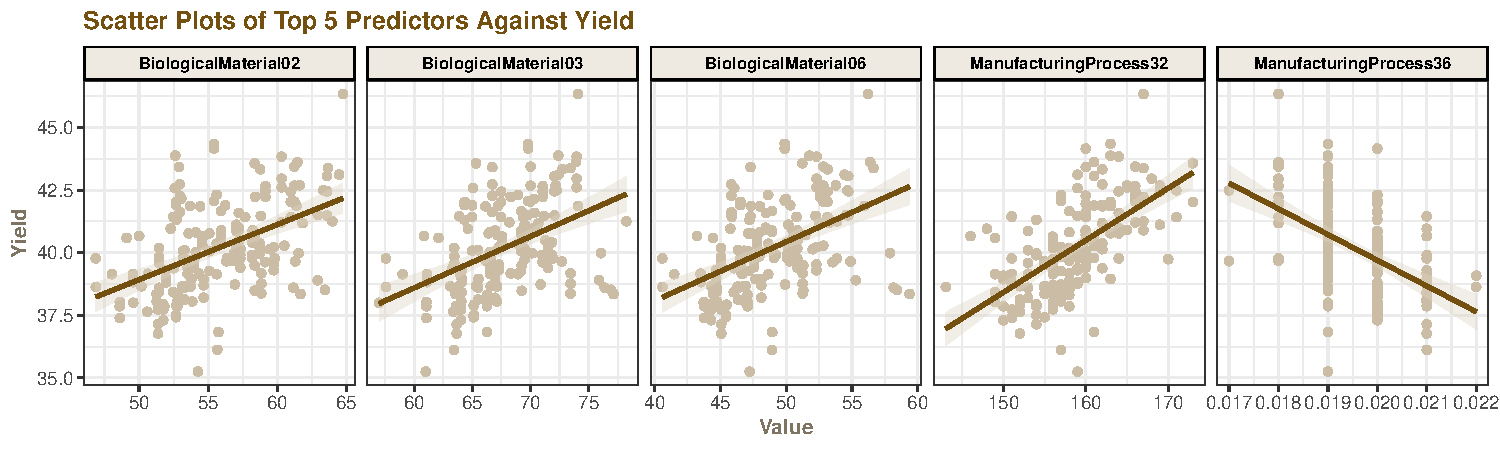
\includegraphics{Homework-Two_files/figure-latex/kj-6.3f-1-1.pdf}

We further examined this relationship by analyzing the correlation
strength between our top five important response variables with the
\texttt{Yield}. Out of which, \texttt{ManufacturingProcess32} showed the
strongest, positive correlation with our response variable.

From a business point of view, our aim is to increase yield since we
know that yield ties into revenue. We do not have insight into what
mechanics go into each manufacturing process but we can use this
knowledge to adjust the processes to emulate the highest yield outputs.

\begin{table}[H]

\caption{\label{tab:kj-6.3f-2}Variable Correlation with Yield}
\centering
\fontsize{8}{10}\selectfont
\begin{tabular}{lr}
\toprule
\textbf{Variable} & \textbf{Yield}\\
\midrule
\rowcolor{gray!6}  ManufacturingProcess32 & 0.6083\\
BiologicalMaterial02 & 0.4815\\
\rowcolor{gray!6}  BiologicalMaterial06 & 0.4782\\
BiologicalMaterial03 & 0.4451\\
\rowcolor{gray!6}  ManufacturingProcess36 & -0.5014\\
\bottomrule
\end{tabular}
\end{table}

\hypertarget{AS-2}{%
\chapter*{Assignment 2}\label{AS-2}}
\addcontentsline{toc}{chapter}{Assignment 2}

\addcontentsline{toc}{subsection}{Kuhn and Johnson 7.2}

\begin{question}{Kuhn and Johnson 7.2}Friedman (1991) introduced several benchmark data sets create by simulation. One of these simulations used the following nonlinear equation to create data: $y = 10\text{sin}(\pi x_1 x_2)+20(x_3-0.5)^2+10x_4+5x_5+N(0\text{,} \sigma^2)$; where the $x$ values are random variables uniformly distributed between $[0, 1]$ (there are also 5 other non-informative variables also created in the simulation). \end{question}

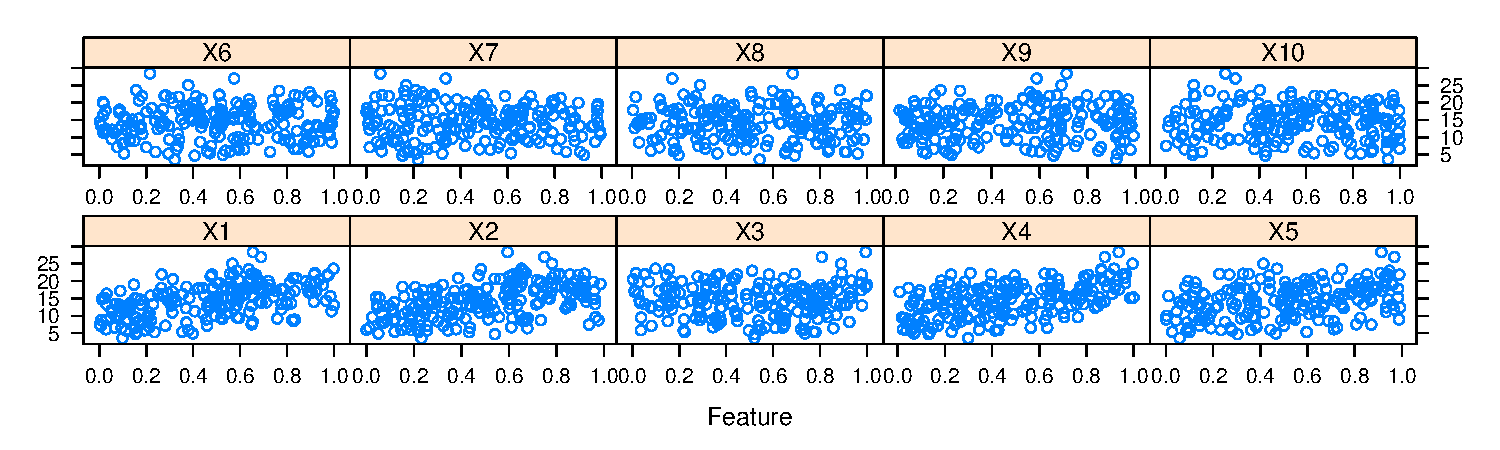
\includegraphics{Homework-Two_files/figure-latex/kj-7.2-ex1-1.pdf}

\begin{subquestion}{(a).} Tune several models on these data. For example: 
\end{subquestion}

Model 1:

Model 2:

Model 3:

\begin{subquestion}{(b).}
Which models appear to give the best performance? Does MARS select the informative predictors (those named X1-X5)?
\end{subquestion}

\addcontentsline{toc}{subsection}{Kuhn and Johnson 7.5}

\begin{question}{Kuhn and Johnson 7.5}
Exercise 6.3 describes data for a chemical manufacturing process. Use the same data imputation, data splitting, and pre-processing steps as before and train several nonlinear regression models.
\end{question}

\begin{subquestion}{(a).}
Which nonlinear regression model gives the optimal resampling and test set performance? 
\end{subquestion}

\begin{subquestion}{(b).}
Which predictors are most important in the optimal nonlinear regression model? Do either the biological or process variables dominate the list? How do the top ten important predictors compare to the top ten predictors from the optimal linear model? 
\end{subquestion}

\begin{subquestion}{(c).}
Explore the relationships between the top predictors and the response for the predictors that are unique to the optimal nonlinear regression model. Do these plots reveal intuition about the biological or process predictors and their relationship with yield?
\end{subquestion}

\hypertarget{AS-3}{%
\chapter*{Assignment 3}\label{AS-3}}
\addcontentsline{toc}{chapter}{Assignment 3}

\addcontentsline{toc}{subsection}{Kuhn and Johnson 8.1}

\begin{question}{Kuhn and Johnson 8.1} Recreate the simulated data from Exercise 7.2: \end{question}

\begin{subquestion}{(a).} Fit a random forest model to all of the predictors, then estimate the variable importance scores. Did the random forest model significantly use the uninformative predictors (V6-V10)?\end{subquestion}

\begin{subquestion}{(b).} Now add an additional predictor that is highly correlated with one of the informative predictors. Fit another random forest model to these data. Did the importance score for V1 change? What happens when you add another predictor that is also highly correlated with V1? For example:\end{subquestion}

\begin{subquestion}{(c).} Use the `cforest` function in the party package to fit a random forest model using conditional inference trees. The party package function `varimp` can calculate predictor importance. The `conditional` argument of that function toggles between the traditional importance measure and the modified version described in Strobl et al. (2007). Do these importances show the same pattern as the traditional random forest model?\end{subquestion}

\begin{subquestion}{(d).} Repeat this process with different tree models, such as boosted trees and Cubist. Does the same pattern occur?\end{subquestion}

\addcontentsline{toc}{subsection}{Kuhn and Johnson 8.2}

\begin{question}{Kuhn and Johnson 8.2}Use a simulation to show tree bias with different granularities.\end{question}

\addcontentsline{toc}{subsection}{Kuhn and Johnson 8.3}

\begin{question}{Kuhn and Johnson 8.3} In stochastic gradient boosting the bagging fraction and learning rate will govern the construction of the trees as they are guided by the gradient. Although the optimal values of these parameters should be obtained through the tuning process, it is helpful to understand how the magnitudes of these parameters affect magnitudes of variable importance. Figure 8.24 provides the variable importance plots for boosting using two extreme values for the bagging fraction (0.1 and 0.9) and the learning rate (0.1 and 0.9) for the solubility data. The left-hand plot has both parameters set to 0.1, and the right-hand plot has both set to 0.9: \end{question}

\begin{subquestion}{(a).} Why does the model on the right focus its importance on just the first few of predictors, whereas the model on the left spreads importance across more predictors? \end{subquestion}

\begin{subquestion}{(b).} Which model do you think would be more predictive of other samples?\end{subquestion}

\begin{subquestion}{(c).} How would increasing interaction depth affect the slope of predictor importance for either model in Fig.8.24?\end{subquestion}

\addcontentsline{toc}{subsection}{Kuhn and Johnson 8.7}

\begin{question}{Kuhn and Johnson 8.7}
Refer to Exercises 6.3 and 7.5 which describe a chemical manufacturing process. Use the same data imputation, data splitting, and pre-processing steps as before and train several tree-based models:
\end{question}

\begin{subquestion}{(a).} Which tree-based regression model gives the optimal resampling and test set performance? \end{subquestion}

\begin{subquestion}{(b).} Which predictors are most important in the optimal tree-based regression model? Do either the biological or process variables dominate the list? How do the top 10 important predictors compare to the top 10 predictors from the optimal linear and nonlinear models?\end{subquestion}

\begin{subquestion}{(c).} Plot the optimal single tree with the distribution of yield in the terminal nodes. Does this view of the data provide additional knowledge about the biological or process predictors and their relationship with yield?\end{subquestion}

\hypertarget{AS-4}{%
\chapter*{Assignment 4}\label{AS-4}}
\addcontentsline{toc}{chapter}{Assignment 4}

\hypertarget{tbd}{%
\section{TBD}\label{tbd}}

\hypertarget{R-Script}{%
\chapter*{R Script}\label{R-Script}}
\addcontentsline{toc}{chapter}{R Script}


\end{document}
